\documentclass[tikz,border=5pt]{standalone}
\usepackage{tikz}
\usetikzlibrary{arrows.meta}
\definecolor{nebula}{HTML}{6366F1}
\definecolor{spark}{HTML}{14B8A6}
\definecolor{ink}{HTML}{334155}
\begin{document}
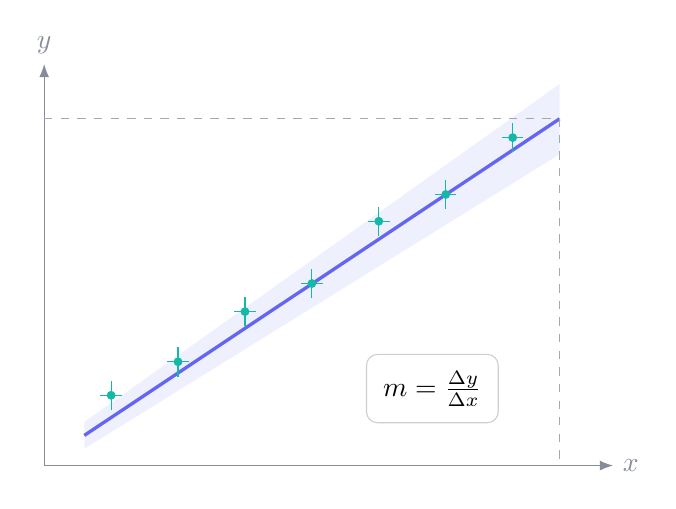
\begin{tikzpicture}[font=\sffamily,>=Latex,x=.85cm,y=.85cm]
  \draw[->,ink!60] (0,0)--(8.5,0) node[right] {$x$};
  \draw[->,ink!60] (0,0)--(0,6) node[above] {$y$};
  \fill[nebula!10] (.6,.65)--(7.7,5.7)--(7.7,4.65)--(.6,.25)--cycle;
  \draw[very thick,nebula] (.6,.45)--(7.7,5.18);
  \foreach \x/\y in {1/1.05,2/1.55,3/2.3,4/2.72,5/3.65,6/4.05,7/4.9}{
    \draw[spark] (\x-.16,\y)--(\x+.16,\y); \draw[spark] (\x,\y-.22)--(\x,\y+.22);
    \fill[spark] (\x,\y) circle (1.6pt);
  }
  \draw[dashed,ink!45] (0,5.18)--(7.7,5.18)--(7.7,0);
  \node[draw=ink!25,rounded corners=4pt,fill=white,inner sep=6pt] at (5.8,1.15)
    {$m=\frac{\Delta y}{\Delta x}$};
\end{tikzpicture}
\end{document}
